%! Author = ASUS
%! Date = 3/6/2023

% Preamble
\documentclass[11pt]{article}

% Packages
\usepackage{amsmath}
\usepackage{wasysym}
\usepackage{graphicx}

\graphicspath{{./images}}

% Document
\begin{document}
    \section{Pinhole Camera}

    A pinhole camera is, basically, consists of a small hole and a plane behind. The light from the real world
    object passes through the hole and forms an inverted and laterally inverted image on the plane which is at
    a distance F from the hole. For the sake of simplicity, it is assumed that there is a virtual screen in front
    of the hole at the same distance F. The same image from the real screen is excepted which is upright if the
    image falls on this virtual screen. The distance between the camera's center and the image plane is known
    as the focal length. The intersection of the optical axis of the lens and the image plane is the principal point.
    These parameters, which characterize the internal geometry of the camera, are known as intrinsic parameters.

    Cameras can have different focal lengths along x and y axes($f_{x} , f_{y}$). And, principal point ($c_{x}, c_{y}$) are
    the coordinates of the optical center in the image plane. The 2D coordinates of a 3D point on the image plane can
    be calculated by similar triangles' equation:

    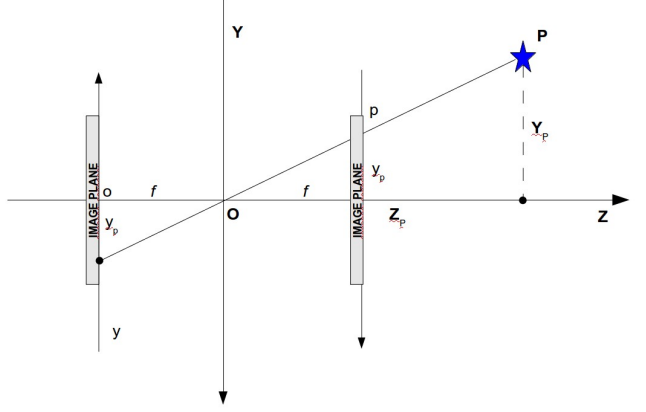
\includegraphics[width=\textwidth,height=\textheight,keepaspectratio]{images/pinhole_2.png}

    \[ x_{p} &= \frac{X_{P}f}{Z_{P}} \quad,\quad y_{p} &= \frac{Y_{P}f}{Z_{P}} \]

    Extrinsic parameters describe how the camera is positioned and oriented in relation to the real world frame.
    The translation \mathbf{t} and rotation \mathbf{R} matrices, and scaling of the camera are some of these parameters.

    a 3D point, is projected onto the image plane, by transforming the point from world coordinate ($X_{w}, Y_{w}, Z_{w}$) system to
    the camera coordinate system using the extrinsic parameters (Rotation \mathbf{R} and Translation \mathbf{t} matrices).
    After having the coordinates of the 3D point from the center of the camera, i.e. ($X_{p}, Y_{p}, Z_{p}$), using the intrinsic parameters
    of the camera, the point is projected onto the image plane. This transformation from world frame to image plane
    is encapsulated in projection matrix.

    \[ \left[
        {\begin{array}{c}
          x_{p} \\
          y_{p} \\
        \end{array}}
    \right]
    &=
    \underbrace{\left[
        {\begin{array}{c}
          \frac{X_{P}f_{x}}{Z_{P}} \\
          \frac{Y_{P}f_{y}}{Z_{P}} \\
        \end{array}}
    \right]}_{\textrm{similar triangle equation}}
    \Rightarrow
    \left[
        {\begin{array}{c}
          X_{P}f_{x} \\
          Y_{P}f_{y} \\
          Z_{P} \\
        \end{array}}
    \right]
    &=
    \left[
        {\begin{array}{cccc}
          f_{x} & 0 & 0 & 0 \\
          0 & f_{y} & 0 & 0 \\
          0 & 0 & 1 & 0 \\
        \end{array}}
    \right]
    \left[
        {\begin{array}{c}
          X_{P} \\
          Y_{P} \\
          Z_{P} \\
          1 \\
        \end{array}}
    \right] \]

    Considering Principal Points $(u_{c}, v_{c})$:

    \[
    \left[
        {\begin{array}{c}
      u \\
      v \\
        \end{array}}
    \right]
    &=
    \left[
        {\begin{array}{c}
      u_{c} + \frac{X_{P}\alpha_{u}}{Z_{p}} \\
      v_{c} + \frac{Y_{P}\alpha_{v}}{Z_{P}} \\
        \end{array}}
    \right]
    \Rightarrow
    \left[
        {\begin{array}{c}
      X_{P}\alpha_{u} + Z_{P}u_{c} \\
      Y_{P}\alpha_{v} + Z_{P}v_{c} \\
      Z_{P} \\
        \end{array}}
    \right]
    &=
    \left[
        {\begin{array}{cccc}
      f_{x} & 0 & u_{c} & 0 \\
      0 & f_{y} & u_{v} & 0 \\
      0 & 0 & 1 & 0 \\
        \end{array}}
    \right]
    \left[
        {\begin{array}{c}
      X_{P} \\
      Y_{P} \\
      Z_{P} \\
      1 \\
        \end{array}}
    \right]
    \]

    Let K be a 3×3 matrix that contains the intrinsic parameters:

    \[
        K
        &=
        \left[
            {\begin{array}{ccc}
          f_{x} & 0 & u_{c} \\
          0 & f_{y} & v_{c} \\
          0 & 0 & 1 \\
            \end{array}}
        \right]
    \]

    Finally, the point P in real world coordinates system is transformed to image plane, u, by:
    \[ u &= K[R|t]P \]

    As it can be seen from the equations, the depth (Z) of the real world points are vanished during the projection.
    In the next sections, we will see how to recover the depth.


    \section{Stereo Cameras}
    \label{stereo_cameras}
    \paragraph{Epipolar geometry}, refers to the geometry of two images of a 3D scene taken
    by two cameras. The two cameras are presumed to have a defined relative pose, which is
    the position and orientation of one camera in relation to the other, and a known internal calibration
    (i.e., focal length, principle point).

    \begin{figure}
        \centering
        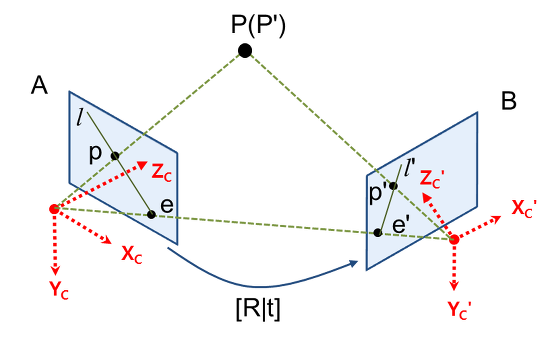
\includegraphics[width=\textwidth,height=\textheight,keepaspectratio]{images/epipolar_1.png}
        \caption{Stereo Cameras}
        \label{fig:stereo_cameras}
    \end{figure}


    \paragraph{Epipolar lines:} Epipolar line is the intersection of the image planes with a plane that
    passes through the two camera centers and a 3D point in the scene. Any point in one image must lie on
    the epipolar line for its equivalent point in the other image. In the figure \ref{fig:stereo_cameras}, l and l' are the epipolar lines.

    \paragraph{Epipoles:} The epipole is the location where the picture planes of the two cameras are
    intersected by the baseline, which connects the centers of the two cameras. To put it another way,
    each camera perceives the epipole of the other camera as a projection of the other camera's center.
    
    \paragraph{Essential Matrix:} Let  $\tilde{p}_l$ and $\tilde{p}_r$ be the vectors from the center of cameras to the points p and p' from figure \ref{fig:stereo_cameras}.
    Recalling translation (t) and rotation (R) matrices, $(t \times R\tilde{p}_r)$  is the cross product vector which is orthogonal to the epipolar plane. Hence,

    \begin{equation}
        \label{eq:1}
        \tilde{p}_l \cdot (t \times R\tilde{p}_r) = 0
    \end{equation}

    Essential matrix is a 3x3 matrix that relates two cameras' poses of two viewpoints. It encodes,
    the relative position and orientation of the two cameras in relation to one another:
    \[ E &= R[t]_{\times} \]
    Where $[t]_{\times}$ is
    \[
        [t]_{\times} &=
        \left[
            {\begin{array}{ccc}
              0 & -t_{3} & t_{2} \\
              t_{3} & 0 & -t_{1} \\
              -t_{2} & t_{1} & 0 \\
            \end{array}}
        \right]
    \]

    By replacing the essential matrix in equation \ref{eq:1}:
    \[ \tilde{p}_l^\top \times E \times \tilde{p}_r &= 0 \]

    Having the linear equation above for a set of corresponded points between two images, essential matrix
    can be calculated. The most common used algorithm to find the essential matrix is known as "Eight-point algorithm".

    In 3D vision problems, once the essential matrix has been calculated, the relative position and orientation
    of the two cameras, i.e. the rotation matrix R and translation vector t, are extracted.
    
    \paragraph{Fundamental Matrix:} A 3x3 matrix that contains not only relative camera poses but also
    camera intrinsic parameters. By having Essential matrix, K and K' as intrinsic camera matrices,
    the fundamental matrix is defined as follows:
    \[ F &= K^{-T} \times E \times K'^{-1}\]
    The same as essential matrix, for points p and p' on image planes:
    \[ p \times F \times p' &= 0 \]

    To calculate the fundamental matrix, the linear equation above can be expanded as follows:
    \begin{equation*}
        p =
        \begin{bmatrix}
            x & y & 1
        \end{bmatrix}
        \text{, }
        F =
        \begin{bmatrix}
        f_{11} & f_{12} & f_{13} \\
        f_{21} & f_{22} & f_{23} \\
        f_{31} & f_{32} & f_{33} \\
        \end{bmatrix}
        \text{, }
        p' =
        \begin{bmatrix}
            x' & y' & 1
        \end{bmatrix}
    \end{equation*}
    \begin{equation*}
        x'xf_{11} + x'yf_{12} + x'f_{13} + y'xf_{21} + y'yf_{22} + y'f_{23} + xf_{31} + yf_{32} + f_{33} = 0 \\
    \end{equation*}

    By rewriting the equation above for multiple correspondence, the homogeneous linear system can be solved using SVD method.

    \section{Two View Geometry}

    \paragraph{Two-view geometry} is the task of finding the relation between two images captured from the same scene
    by two cameras with different viewpoints, and detecting the 3D position of points in the scene. We start by
    detecting the depth of a pixel with basic geometry calculus, and then, generalize it to all possible camera settings.

    \paragraph{Rectilinear Rig} Starting with two cameras with the same intrinsic parameters with parallel baseline, i.e. the planes of
    two cameras are aligned in one line as shown in figure \ref{fig:rect_rig}, By using similar triangles equations,
    the depth of a keypoint can be calculated:

    \begin{figure}
        \centering
        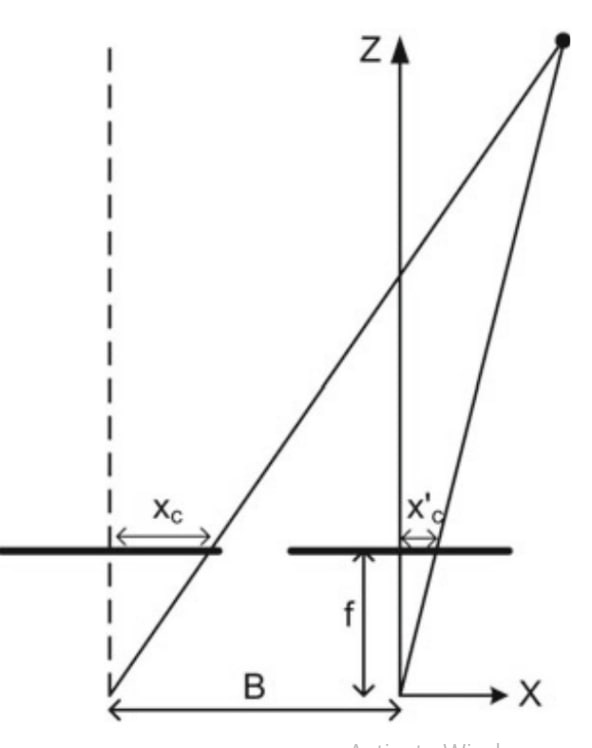
\includegraphics[scale=0.5]{images/two_view}
        \caption{Rectilinear Rig}
        \label{fig:rect_rig}
    \end{figure}

    \[ x'_{c} &= f\frac{X}{Z} \quad,\quad x_{c} &= f\frac{X+B}{Z} \]
    \[ d &= x_{c} - x'_{c} &= \frac{fB}{Z} \]
    \[ Z &= \frac{fB}{d} \]

    Let d, from the equation above, called the disparity which is the difference in the coordinates of the pixels in both images pointing to the same 3D point.
    Therefore, the only challenge is to find the disparity of each pixel.

    \paragraph{For other camera settings}, e.g. non-parallel baselines, different camera parameters,
    the fundamental matrix is the key option that can be used to find the depth of points.
    A 3D point can be defined as the intersection of the rays that start from the centers of cameras and
    cross the corresponded 2D keypoints in each image plane. In practice, first, the fundamental and the essential
    matrices are calculated by finding the accurate feature matches between
    the two images. Then, after having the relative pose of cameras, for all pixels, the corresponding pixel from the other image is found along the epipolar lines.
    The epipolar lines help to limit the search space for matching process from all pixels over the images to only the pixels
    on epipolar line and its surroundings. By having camera poses and all matches, 3D points could be obtained by triangulation.

    \section{Camera Distortion and Calibration}

    \paragraph{Distortion} refers to the deviation between the ideal pinhole camera model and the actual camera
    used to capture images. The pinhole camera model assumes that light rays pass through a single point, or
    the pinhole, before forming an image on a flat image plane. However, real-world cameras have imperfect
    lenses, that doesn't let rays reflect straightly and causes distortions to the image.

    There are two kinds of camera distortions:

    \begin{enumerate}
        \item Radial distortion is caused by the curvature of the camera lens. This type of distortion
        causes straight lines to appear curved in the image, especially near the edges of the image.
        \item Tangential distortion occurs when the lens is not aligned perfectly parallel to the image plane.
        This causes the image to appear skewed, with some parts appearing closer or farther from the camera
        than they should.
    \end{enumerate}
    {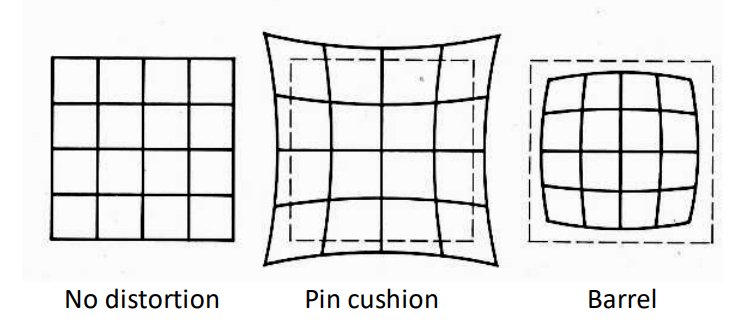
\includegraphics[width=\textwidth,height=\textheight,keepaspectratio]{distortion.PNG}}

    \paragraph{Camera calibration} is the process of estimating the intrinsic parameters like focal length,
    principal point, and distortion coefficients, as well as the extrinsic parameters like camera position
    and orientation for each image. The accuracy of this step has significant impact on 3D reconstruction.
    As it is mentioned in previous sections, the depth of a pixel has direct relation with focal length. The depth
    can be in meters, while focal length is usually around millimeters. Therefore, a small error in focal length
    can cause high misplacement of a 3D point's position.

    \paragraph{Homography:} Let there be two images from the same planar scene, e.g. a rectangular identity card, but from
    different viewpoints. The second view can be obtained from the first view by multiplying the first image by
    a 3x3 matrix called Homography matrix.

    A checkerboard is used to take pictures of for calibration since it is a planar object and it has distinctive features,
    i.e. checkerboard corners, that are easy to detect. A set of pictures are taken from different point of views.
    By using homography, an initial guess for intrinsic parameters are calculated. Then, the final calibration
    parameters are refined by optimizing the reporjection equations for checkerboard corners.

\end{document}
